%
% main.tex -- Paper zum Thema <fourier>
%
% (c) 2020 Autor, OST Ostschweizer Fachhochschule
%
% !TEX root = ../../buch.tex
% !TEX encoding = UTF-8
%
\chapter{Fourier-Transformation und Feldtheorie\label{chapter:fourier}} % todo: Titel: Fourier & Quantentheorie?
\kopflinks{Fourier-Transformation und Feldtheorie}
\begin{refsection}
\chapterauthor{Martina Knobel, Gian Kraus}

Ein paar Hinweise für die korrekte Formatierung des Textes
\begin{itemize}
\item
Absätze werden gebildet, indem man eine Leerzeile einfügt.
Die Verwendung von \verb+\\+ ist nur in Tabellen und Arrays gestattet.
\item
Die explizite Platzierung von Bildern ist nicht erlaubt, entsprechende
Optionen werden gelöscht. 
Verwenden Sie Labels und Verweise, um auf Bilder hinzuweisen.
\item
Beginnen Sie jeden Satz auf einer neuen Zeile. 
Damit ermöglichen Sie dem Versionsverwaltungssysteme, Änderungen
in verschiedenen Sätzen von verschiedenen Autoren ohne Konflikt 
anzuwenden.
\item 
Bilden Sie auch für Formeln kurze Zeilen, einerseits der besseren
Übersicht wegen, aber auch um GIT die Arbeit zu erleichtern.
\end{itemize}

%
% einleitung.tex -- Einleitung und Motivation
%
% (c) 2020 Prof Dr Andreas Müller, Hochschule Rapperswil
%
% !TEX root = ../../buch.tex
% !TEX encoding = UTF-8
%

\section{Einleitung\label{fourier:section:einleitung}}
%\kopfrechts{Grundlagen der Fourier-Analyse}


Felder kann man sich als eine unendliche Ansammlung von Feldlinien vorstellen, die sich kreuz und quer durch Raum-Zeit schlängeln. Die Fourier-Analyse hilft dabei, dieses scheinbare Chaos in einfache Sinus- und Cosinus-Schwingungen zu zerlegen. 
In der Quantenfeldtheorie werden diese Schwingungen anders interpretiert, was letztlich dazu führt, dass das Feld als Summe einer beschränkten Anzahl von Teilen verstanden wird.










%
% fourierGrundlagen.tex -- Mathematische Grundlagen der Fourier Reihe & Transformation
%
% (c) 2020 Prof Dr Andreas Müller, Hochschule Rapperswil
%
% !TEX root = ../../buch.tex
% !TEX encoding = UTF-8
%

\section{Fourierreihe\label{fourier:section:GrundlagenFourierAnalyse}}
\kopfrechts{Fourierreihe}


Mit der Fourier-Reihe lassen sich periodisch wiederholende Funktionen, wie ein Rechteck- oder Dreiecksignal, mit skalierten Sinus- und Kosinusschwingungen darstellen. 
Um die Reihe aufzustellen, braucht man nur drei Arten von Koeffizienten zu bestimmen. 

\begin{itemize}
	\item $a_0$ ist der Mittelwert, der Funktion. 
	Dieser entspricht dem Integral über eine Periode und schliesslich geteilt durch die Periode: 
	
	\begin{equation}
		a_0 = \frac{1}{T} \int_{t_0}^{t_0 + T} f(t) \, dt
	\end{equation}
	
	\item Die $a_n$ definieren den geraden Anteil der Funktion:
	
	\begin{equation}
		a_n = \frac{2}{T} \int_{t_0}^{t_0 + T} f(t) \cos\left(\frac{2\pi n t}{T}\right) dt
	\end{equation}
	
	\item Die $b_n$ definieren den ungeraden Anteil der Funktion:
	
	\begin{equation}
		b_n = \frac{2}{T} \int_{t_0}^{t_0 + T} f(t) \sin\left(\frac{2\pi n t}{T}\right) dt
	\end{equation}
	
\end{itemize}


Mit allen Koeffizienten bestimmt und genügend Zeit um unendlich Summen zu berechnen lassen sich fast alle Funktionen perfekt approximieren.
Die $a_n$ und $b_n$ skalieren die Amplituden der Schwingungen, in abhängigkeit zu $n>=1$. 
Je nach Funktion können diese Faktoren durchaus komplizierte funktionen annehmen.
Generell nimmt die Amplituden mit höherem $n$ ab, ob linear, quadratisch oder mit dem Kehrwert von n lässt sich Allgemein nicht bestimmen.
Mit jeder iteration der Summe steigt die Frequenz linear an.
Das ist die Fourier-Reihe:


\begin{equation}
f(t) = \frac{a_0}{2} + \sum_{n=1}^{\infty} \left( a_n \cos\left( \frac{2\pi n}{T} t \right) + b_n \sin\left( \frac{2\pi n}{T} t \right) \right)
\end{equation}


Die Ausnaheme sind Funktionen mit Sprungstellen, wie in Abbildung \ref{fourier:fourierrechteck}.
Bei dieser Rechteckfunktion wurden die Reihe bis $n = 3$ berechnet. 
Bei solchen Funktionen tritt das sogenannte Gibbsche Phänomen auf.
In der Nähe eines Sprungs entsteht ein charakteristischer Überschwinger, der selbst bei unendlich vielen Summanden nicht verschwindet.
Das Gleichheitszeichen $=$ gilt daher nur eingeschränkt. 
Nun folgen zwei Bespiele.



\begin{figure}[H]
	\centering
	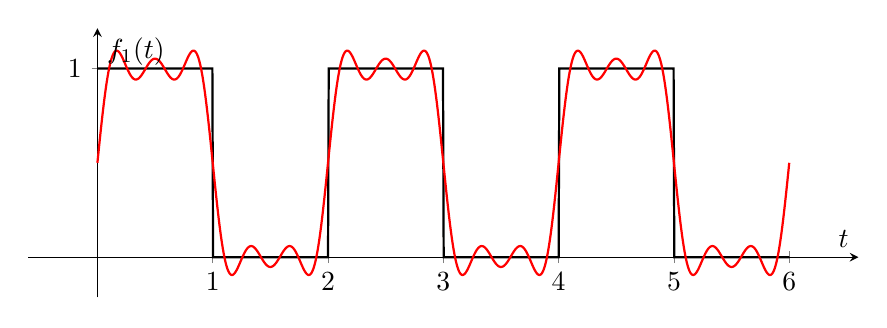
\begin{tikzpicture}
		\begin{axis}[
			axis lines = middle,
			xlabel = {$t$},
			ylabel = {$f_1(t)$},		
			domain=0:6,
			samples=1000,
			xtick={0,1,2,3,4,5,6},
			ytick={0,1},
			enlargelimits,
			width=\textwidth,
			height=5cm
			]
			\addplot[thick] {mod(floor(x),2) == 0 ? 1 : 0};
			\addplot[red, thick] {(1/2) + 
				(2/pi)*sin(pi * deg(x)) + 
				(2/(3*pi))*sin(pi *3*deg(x)) +
				(2/(5*pi))*sin(pi *5*deg(x))};
		\end{axis}
	\end{tikzpicture}
	\caption{Fourierapproximation einer Rechteckfunktion}
	\label{fourier:fourierrechteck}
\end{figure}

\begin{equation}
	f_1(t) = \frac{1}{2} + \sum_{\substack{n=1 \\ n\ \text{ungerade}}}^{5} \frac{1}{\pi n^2} \sin\left( \pi n t \right)
\end{equation}

$f_1(t)$ entspricht der roten Funktion. 
Der Mittelwert $a_0$ entspricht $\frac{1}{2}$. 
Die Rechteck Funktion ist abzüglich $a_0$ eine ungerade Funktion, da gilt $f_1(t) = -f_1(t)$. 
Daher ist der gerade Anteil $a_n$ stets Null. 
Zudem wurde noch eine vereinfachung von $b_n$ vorgenommen, da der Term bei geraden $n$ Null wird, summiert man nur über ungerade $n$. 


\begin{figure}[H]
	\centering
	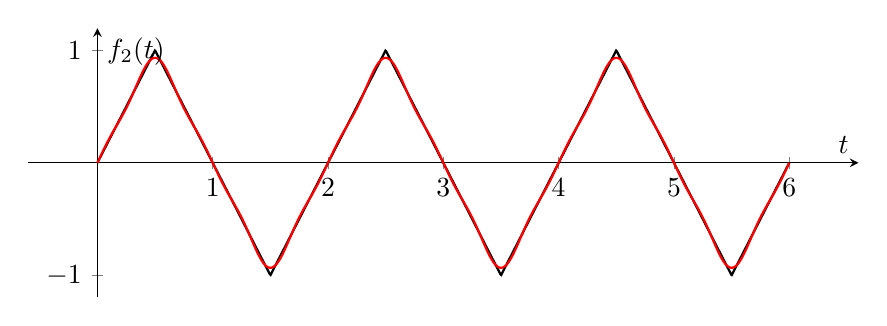
\begin{tikzpicture}
		\begin{axis}[
			axis lines = middle,
			xlabel = {$t$},
			ylabel = {$f_2(t)$},		
			domain=0:6,
			samples=1000,
			xtick={0,1,2,3,4,5,6},
			ytick={-1,0,1},
			enlargelimits,
			width=\textwidth,
			height=5cm
			]
			\addplot[black, thick] {
				abs(mod(x+0.5,2) - 1) * (-2) + 1
			};
			
			\addplot[red, thick, domain=0:6] {
				(8/pi^2) * (
				sin(deg(pi*x))/1^2
				- sin(deg(3*pi*x))/3^2
				+ sin(deg(5*pi*x))/5^2
				)
			};
		\end{axis}
	\end{tikzpicture}
	\caption{Fourierapproximation einer Dreieckfunktion}
	\label{fourier:fourierdreieck}
\end{figure}

\begin{equation}
	f_2(t) = \sum_{\substack{n=1 \\ n\ \text{ungerade}}}^{5} \frac{8}{\pi^2 n^2} \cos(n\pi t)
\end{equation}

$f_2(t)$ entspricht der roten Funktion und überdeckt das Orginal beinahe perfekt. 
Dies mit nur drei Iterationen!
Der Mittelwert ist $a_0$ ist hier 0. 
Die Dreieck Funktion ist eine gerade Funktion, da gilt $f_1(t) = f_1(-t)$. 
Daher ist der ungerade Anteil $a_n$ stets Null. 
Wie beim ersten Beispiel wurde $b_n$ vereinfacht, man summiert nur über ungerade $n$. 


Bei der Fourier-Reihen Bildung kann man sich viel Zeit erspaaren, wenn man zuerst überprüft ob es sich um eine gerade oder ungerade Funktion handelt.
So kann man ohne zu rechnen $a_n$ oder $b_n$ gleich Null setzen.

%bei der Quantenmechanik rechnet man stets komplex. maybe noch erwähnen: die komplexe Fourierreihe




%
% anwendungenFelder.tex -- 3.	Anwendungen auf Felder, PDEs in ODE umwandeln (Grundlage, um Feldgleichungen als eine Familie von Oszillator-Gleichungen zu interpretieren)
%
% (c) 2020 Prof Dr Andreas Müller, Hochschule Rapperswil
%
% !TEX root = ../../buch.tex
% !TEX encoding = UTF-8
%

%    Anwendungen auf Felder, PDEs in ODE umwandeln (Grundlage, um Feldgleichungen als eine Familie von Oszillator-Gleichungen zu interpretieren) 


\section{Anwendung auf Feld\label{fourier:section:AnwendungAufFeld}}
\kopfrechts{Anwendung auf Feld}
%Motivation. E & B Felder enfüllen wellengleichung. noch schreiben!
Gewöhnliche Differentialgleichungen sind berühmt berüchtigt schwierig zu lösen.
Schlimmer geht es immer.
Partielle Differenzialgleichungen enthaltet Ableitungen nach mehreren Variabeln.
In diesem Abschnitt vereinfachen wir eine partielle Differentialgleichung, mithilfe der Fourierreihe, in eine Gewöhnliche.
Alle Ableitungen müssen schlussendlich den identischen Nenner besitzen. 
Im unteren Beispiel ist das die Zeit $\partial t$.
Als partielle Differentialgleichung verwenden wir die eindimensionale Wellengleichung mit der Lichtgeschwindigkeit als Ausbreitungsgeschwindigkeit. 
Dieses Modell eignet sich besonders gut, da es auch auf elektromagnetische Felder anwendbar ist!

\begin{equation}
	\frac{\partial^2 u(x, t)}{\partial t^2} = c^2 \cdot \frac{\partial^2 u(x, t)}{\partial x^2}
\end{equation}

Unter der Annahme, dass $u(x, t)$ eine sich periodisch wiederholende Funktion ist, führen wir eine Fourierreihen-Entwicklung durch. 
Neu besteht $u(x, t)$ aus einer unendlichen Anzahl von Schwingungen:

\begin{equation}
	u(x,t) = \frac{a_0(t)}{2} + \sum_{n=1}^{\infty} \left( a_n(t) \cos(n \omega x) + b_n(t) \sin(n \omega x) \right)
\end{equation}

Alle drei Fourier Koeffizienten erhält man durch die integral-Rechnungen im Abschnitt \ref{fourier:section:GrundlagenFourierAnalyse}. 
Da das Ziel ist, $x$ zu eliminieren, integriert man über eine Periode nach $x$.
Somit entstehen Fourier-Koeffizienten, die von $t$ abhängig sind. 
Nun wird $u(x,t)$ in seiner Summenform in die Wellengleichung eingebaut. 
Dazu muss $u(x,t)$ je zwei Mal nach $t$ und $x$ abgeleitet werden:

\begin{equation}
	\frac{\partial^2 u(x,t)}{\partial t^2} = \frac{1}{2} \frac{\partial^2 a_0(t)}{\partial t^2} +  \sum_{n=1}^{\infty} \left( \frac{\partial^2}{\partial t^2} a_n(t) \cos(n \omega x) + \frac{\partial^2}{\partial t^2} b_n(t) \sin(n \omega x) \right)
\end{equation}

\begin{equation}
	\frac{\partial^2 u(x,t)}{\partial x^2} = \sum_{n=1}^{\infty} \left( -a_n(t) n^2 \omega^2 \cos(n \omega x) - b_n(t) n^2 \omega^2 \sin(n \omega x) \right)
\end{equation}


Von nun an, wird als ableitungsoperator $\frac{d}{dt}$ verwendet, da die Gleichung nur noch von $t$ abhängig ist.
Die Resultate können jetzt in die Wellengleichung einsetzt werden. 

%\begin{equation}
%	 \frac{1}{2} \frac{d^2 a_0(t)}{d t^2} + \sum_{n=1}^{\infty} \left( \frac{d^2}{dt^2} a_n(t) \cos(n \omega x) + \frac{d^2}{dt^2} b_n(t) \sin(n \omega x) \right) = c^2  \sum_{n=1}^{\infty} \left( -a_n(t) n^2 \omega^2 \cos(n \omega t) - b_n(t) n^2 \omega^2 \sin(n \omega t) \right) 
%\end{equation}


\begin{multline}
	\frac{1}{2}\frac{\partial^2 a_0(t)}{dt^2}
	+ \sum_{n=1}^{\infty}\Bigl(
	\frac{d^2 a_n(t)}{dt^2}\cos(n\omega x)
	+ \frac{d^2 b_n(t)}{dt^2}\sin(n\omega x)
	\Bigr)
	= \\[-0.8ex]
	c^2 \sum_{n=1}^{\infty}\Bigl(
	-a_n(t)\,n^2\omega^2\cos(n\omega x)
	-b_n(t)\,n^2\omega^2\sin(n\omega x)
	\Bigr)
\end{multline}


Diese etwas grosse Gleichung kann nun mithilfe eines Koeffizientenvergleichs gelöst werden.
So entstehen folgende drei Gleichungen:

\begin{equation}
	\frac{1}{2} \frac{d^2 a_0(t)}{d t^2} = 0
\end{equation}

\begin{equation}
	\sum_{n=1}^{\infty}
	\frac{d^2 a_n(t)}{dt^2}\cos(n\omega x)
	 = c^2 \sum_{n=1}^{\infty}
	-a_n(t)\,n^2\omega^2\cos(n\omega x)
	\end{equation}

\begin{equation}
	\sum_{n=1}^{\infty}
	\frac{d^2 b_n(t)}{dt^2}\sin(n\omega x) = c^2 \sum_{n=1}^{\infty}
	-b_n(t)\,n^2\omega^2\sin(n\omega x)
\end{equation}


Die zweite Ableitung des Mittelwerts $a_0(t)$ ist 0, somit ist $a_0(t)$ eine Gerade, eine Konstante oder 0. Also ist $a_0(t)$ von der Form $a_0(t)=C_1 t + C_2$. 
$C_1$ und $C_2$ sind Integrationskonstanten.



Die Gleichungen mit $a_n(t)$ und $b_n(t)$ kann man wiederrum mit einem Koefizientenvergleich lösen, diesmal jedoch über eine unendliche Summe! Man endet mit einer unendlichen anzahl von Gleichungen für jede Frequenz. Da sie alle dieselbe Form haben, bleibt man mit der schreibweise mit $n$.
Zudem sind die $\cos(n\omega x)$ und $\sin(n\omega x)$ zu kürzen. 
Somit entstehen folgende zwei gewöhnliche Differentialgleichungen:

\begin{equation}
	\frac{d^2}{dt^2} a_n(t) + a_n(t) n^2 \omega^2 c^2 = 0
	  \quad   \text{und} \quad  \frac{d^2}{dt^2} b_n(t) + b_n(t) n^2 \omega^2 c^2 = 0
\end{equation}

Falls man im Physik unterricht aufgepasst hat, sollte einem diese Form bekannt vorkommen. Die Differentialgleichung einem ungedämpften Federpendels besitzt dieselbe Form. 

\begin{equation}
	\frac{d^2}{dt^2} x(t) + x(t) \omega^2  = 0
\end{equation}

Die lösung von dieser Gleichung ist einfach eine ungedämpfte schwingung der Form 

\begin{equation}
x(t) = A \cos(\omega t) + B \sin(\omega t) \quad \text{oder} \quad x(t) = C \cos(\omega t - \varphi)
\end{equation}

Dieses Resultat beschreibt mit welcher Frequenz und Amplitude eine Masse an einer Feder schwingt. 

Könnte man nun dasselbe mit der resultierenden Lösung der Wellengleichung machen?
Das Resultat wäre eine unendliche Anzahl von Felderpendeln, da $n$ für jede natürliche Zahl steht. 
Die Kreisfrequenz wäre  $n \omega c$. 
Dies macht mathematisch Sinn, physikalisch müsste man sich jedoch fragen, was genau hin und her pendelt und ob eine unendliche Frequenz möglich ist?



In diesem Kapitel wurde die Thematik vereinfacht dargestellt. 
Anstelle eines dreidimensionales Feldes $u(x,y,z,t)$ wurde lediglich eine eindimensionale Funktion $u(x,t)$ betrachtet. Die Fourier-Reihe lässt sich auch auf mehrdimensionale Felder anwenden, der damit verbundene mathematische Aufwand ist jedoch höher. 









%
% quantenfeldtheorie.tex -- Quantenfeldtheorie:  Quantisierung, Schrödinger-Gleichung, der harmonische Oszillator, Photonen als Oszillatoren
%
% (c) 2020 Prof Dr Andreas Müller, Hochschule Rapperswil
%
% !TEX root = ../../buch.tex
% !TEX encoding = UTF-8
%
\section{Quantenfeldtheorie
\label{fourier:section:quantenfeldtheorie}}
\kopfrechts{Quantenfeldtheorie}
Zunächst erfolgt ein Exkurs in die Quantentheorie, um schliesslich zum Laser zu gelangen. % Todo überarbeiten; evtl. weglassen

...
Energie wird in Form von Quanten gespeichert.
Vielfache der Grundfrequenz sind möglich.

Elektromagnetisches Feld $\rightarrow$ Fourier $\rightarrow$ Feldgleichung wie Gleichung vom Federpendel

\subsection{Der harmonische Oszillator
\label{fourier:subsection:derHarmonischeOszillator}}
Warum genau schauen wir uns den harmonischen Oszillator an?
In der Quantenelektrodynamik werden die elektromagnetischen Felder als quantisierte harmonische Oszillatoren modelliert, deren Energie ebenfalls in Vielfachen von $\hbar\cdot\omega$ vorliegt.
Die Zustände des Feldes (Photonenzahlenzustände) werden durch die Schwingungszustände des harmonischen Oszillators beschrieben.

Diese Quantisierung erklärt, warum Licht in Lasern nicht kontinuierlich, sondern in diskreten Paketen (Photonen) emittiert wird. % todo: diesen Satz an anderer passenden Stelle einfügen

Die Wellengleichung lautet bekanntlich
\begin{equation}
    \frac{\partial^2 u}{\partial t^2} = c^2 \left( \frac{\partial^2 u}{\partial x^2} + \frac{\partial^2 u}{\partial y^2} \right).
\end{equation}
Wenn nun der y-Anteil als konstant betrachtet wird, sind alle partiellen Ableitungen nach y gleich Null.
Dies führt zu der vereinfachten Gleichung
\begin{equation}
    \frac{\partial^2 u}{\partial t^2} = c^2 \frac{\partial^2 u}{\partial x^2}.
\end{equation}
Daraus lässt sich die Differentialgleichung
\begin{equation}
    \ddot{a}(t) = -k^2 a(t)
\end{equation}
aufstellen.
$a(t)$ ist hierbei ein Fourier-Koeffizient des elektromagnetischen Wellenfeldes.
Die Lösung dieser Differentialgleichung lautet
\begin{equation}
    u(t,x) = a_k(t) \cos(kx)
\end{equation}

% Besser sin verwenden --> besser e^ikx verwenden; Überlegen, ob wir komplex arbeiten möchten
% In Präsentation mit cos und im Paper mit e^ikx


% Wichtiger Schritt: Der harmonische Oszillator in der Quantenmechanik --> Unterlagen anschauen. 
% Evtl. Termin mit ihm, um Unklarheiten zu klären.

Diese Gleichung ist analog zur Gleichung eines Federpendels.
Es handelt sich hier um ein "Quanten-Federpendel".
% \begin{tikzpicture}

%     % Zeichne die horizontale Linie (Boden)
%     \draw[thick] (-2,0) -- (2,0);
    
%     % Zeichne die Wand
%     \draw[thick] (0,0) -- (0,2);
    
%     % Zeichne die Feder
%     \draw[thick] (0,2) -- (0,4);
%     \draw[thick] (0,4) -- (0.5,4.5);
%     \draw[thick] (0.5,4.5) -- (0,5);
    
%     % Zeichne die Masse
%     \filldraw[fill=gray] (0,5) circle (0.2);
    
%     % Zeichne die Schnur
%     \draw[thick] (0,5) -- (0,6);
    
%     \end{tikzpicture} % unschönes bild, sollte ein Federpendel werden; todo
% todo: weiterschreiben

%\input{papers/fourier/laser.tex} % todo: evtl. ganz weglassen?

\printbibliography[heading=subbibliography]
\end{refsection}
